%!TEX program = pdflatex
\documentclass[aspectratio=169,9pt]{beamer}

% Minimal theme - clean
\usetheme{default}
\usecolortheme{default}
\setbeamertemplate{navigation symbols}{}
\setbeamertemplate{footline}[frame number]

% Colors
\definecolor{primary}{RGB}{41, 65, 114}
\definecolor{secondary}{RGB}{76, 114, 176}
\definecolor{accent}{RGB}{255, 140, 0}
\definecolor{lightblue}{RGB}{235, 245, 255}
\definecolor{lightgray}{RGB}{250, 250, 252}
\definecolor{darkgray}{RGB}{50, 50, 60}

\setbeamercolor{frametitle}{fg=primary}
\setbeamercolor{title}{fg=primary}
\setbeamercolor{footline}{fg=gray}

% Packages
\usepackage{tikz}
\usetikzlibrary{shapes.geometric, arrows.meta, positioning, calc, fit, backgrounds}
\usepackage{amsmath}

% TikZ Styles - smaller and cleaner
\tikzset{
    box/.style={
        rectangle, rounded corners=3pt, 
        minimum width=1.4cm, minimum height=0.55cm,
        draw=#1, fill=#1!15, text=darkgray, 
        font=\tiny, align=center, line width=0.6pt
    },
    bigbox/.style={
        rectangle, rounded corners=5pt,
        minimum width=2cm, minimum height=0.7cm,
        draw=#1, fill=#1!20, text=darkgray,
        font=\tiny\bfseries, align=center, line width=1pt
    },
    arrow/.style={-Stealth, thick, color=primary},
    dashedarrow/.style={-Stealth, dashed, color=secondary},
    anno/.style={font=\tiny, text=darkgray}
}

\begin{document}

%===============================================================================
% SLIDE 1: System Architecture - Main Pipeline
%===============================================================================
\begin{frame}
\frametitle{\textbf{τ-Diffusion: System Architecture}}
\vspace{-0.5cm}
\begin{center}
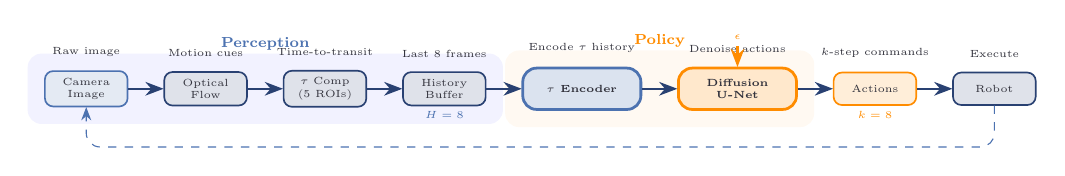
\begin{tikzpicture}[node distance=0.4cm and 0.6cm, scale=0.75, transform shape]
    
    % Row 1: Perception
    \node[box=secondary] (cam) {Camera\\Image};
    \node[box=primary, right=of cam] (of) {Optical\\Flow};
    \node[box=primary, right=of of] (tau) {$\tau$ Comp\\(5 ROIs)};
    \node[box=primary, right=of tau] (buf) {History\\Buffer};
    
    % Row 1: Policy
    \node[bigbox=secondary, right=of buf] (enc) {$\tau$ Encoder};
    \node[bigbox=accent, right=of enc] (diff) {Diffusion\\U-Net};
    \node[box=accent, right=of diff] (act) {Actions};
    \node[box=primary, right=of act] (robot) {Robot};

    % Short block explanations
    \node[anno, above=0.12cm of cam] {Raw image};
    \node[anno, above=0.12cm of of] {Motion cues};
    \node[anno, above=0.12cm of tau] {Time-to-transit};
    \node[anno, above=0.12cm of buf] {Last 8 frames};
    \node[anno, above=0.12cm of enc] {Encode $\tau$ history};
    \node[anno, above=0.12cm of diff] {Denoise actions};
    \node[anno, above=0.12cm of act] {$k$-step commands};
    \node[anno, above=0.12cm of robot] {Execute};
    
    % Arrows
    \draw[arrow] (cam) -- (of);
    \draw[arrow] (of) -- (tau);
    \draw[arrow] (tau) -- (buf);
    \draw[arrow] (buf) -- (enc);
    \draw[arrow] (enc) -- (diff);
    \draw[arrow] (diff) -- (act);
    \draw[arrow] (act) -- (robot);
    
    % Feedback
    \draw[dashedarrow, rounded corners=5pt] (robot.south) -- ++(0,-0.7) -| (cam.south);
    
    % Noise
    \draw[arrow, color=accent] ($(diff.north)+(0,0.35)$) -- (diff.north);
    \node[font=\tiny, color=accent] at ($(diff.north)+(0,0.5)$) {$\epsilon$};
    
    % Labels
    \node[font=\tiny, text=secondary] at ($(buf.south)+(0,-0.15)$) {$H=8$};
    \node[font=\tiny, text=accent] at ($(act.south)+(0,-0.15)$) {$k=8$};
    
    % Background groups
    \begin{scope}[on background layer]
        \node[fit=(cam)(of)(tau)(buf), fill=blue!5, rounded corners=5pt, inner sep=6pt] (g1) {};
        \node[fit=(enc)(diff), fill=orange!5, rounded corners=5pt, inner sep=6pt] (g2) {};
    \end{scope}
    
    \node[font=\scriptsize\bfseries, text=secondary] at ($(g1.north)+(0,0.15)$) {Perception};
    \node[font=\scriptsize\bfseries, text=accent] at ($(g2.north)+(0,0.15)$) {Policy};
    
\end{tikzpicture}
\end{center}

\vspace{0.2cm}

% ROI Diagram - separate section
\begin{columns}[T]
\begin{column}{0.35\textwidth}
\centering
\textbf{\small 5 Region-of-Interest (ROI)}

\vspace{0.15cm}

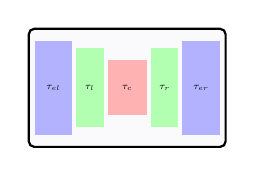
\begin{tikzpicture}[scale=0.5, transform shape]
    \draw[thick, fill=lightgray, rounded corners=2pt] (0,0) rectangle (5,3);
    
    % ROIs with clear labels
    \fill[blue!30] (0.15,0.3) rectangle (1.1,2.7);
    \node[font=\scriptsize] at (0.625,1.5) {$\tau_{el}$};
    
    \fill[blue!30] (3.9,0.3) rectangle (4.85,2.7);
    \node[font=\scriptsize] at (4.375,1.5) {$\tau_{er}$};
    
    \fill[green!30] (1.2,0.5) rectangle (1.9,2.5);
    \node[font=\scriptsize] at (1.55,1.5) {$\tau_l$};
    
    \fill[green!30] (3.1,0.5) rectangle (3.8,2.5);
    \node[font=\scriptsize] at (3.45,1.5) {$\tau_r$};
    
    \fill[red!30] (2.0,0.8) rectangle (3.0,2.2);
    \node[font=\scriptsize] at (2.5,1.5) {$\tau_c$};
\end{tikzpicture}
\end{column}

\begin{column}{0.6\textwidth}
\textbf{\small Key Parameters}
\begin{itemize}\setlength{\itemsep}{1pt}
    \item[\tiny$\bullet$] \footnotesize $\tau \in \mathbb{R}^5$: Time-to-Transit per ROI
    \item[\tiny$\bullet$] \footnotesize History buffer: $H = 8$ frames
    \item[\tiny$\bullet$] \footnotesize Action horizon: $k = 8$ steps
    \item[\tiny$\bullet$] \footnotesize Diffusion: 100 train / 10 inference steps
\end{itemize}
\end{column}
\end{columns}
\end{frame}

%===============================================================================
% SLIDE 2: DAgger Training Loop
%===============================================================================
\begin{frame}
\frametitle{\textbf{Training Pipeline: DAgger Algorithm}}
\vspace{-0.3cm}
\begin{center}
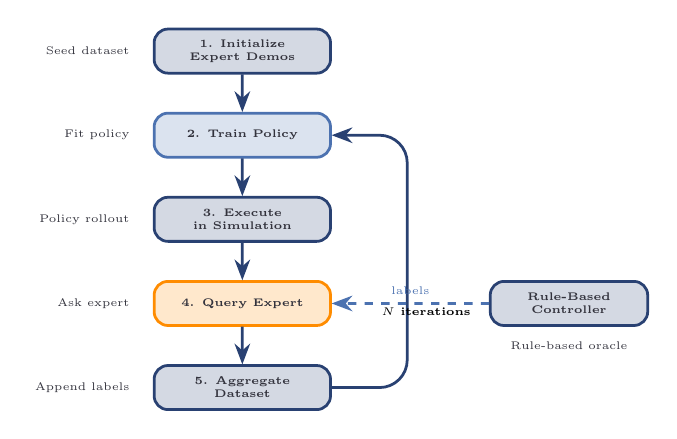
\begin{tikzpicture}[node distance=0.6cm, scale=0.8, transform shape]
    
    % Main loop nodes - vertical
    \node[bigbox=primary, minimum width=2.8cm] (init) {1. Initialize\\Expert Demos};
    
    \node[bigbox=secondary, below=of init, minimum width=2.8cm] (train) {2. Train Policy};
    
    \node[bigbox=primary, below=of train, minimum width=2.8cm] (roll) {3. Execute\\in Simulation};
    
    \node[bigbox=accent, below=of roll, minimum width=2.8cm] (query) {4. Query Expert};
    
    \node[bigbox=primary, below=of query, minimum width=2.8cm] (agg) {5. Aggregate\\Dataset};

    % Short block explanations
    \node[anno, anchor=east] at ($(init.west)+(-0.25,0)$) {Seed dataset};
    \node[anno, anchor=east] at ($(train.west)+(-0.25,0)$) {Fit policy};
    \node[anno, anchor=east] at ($(roll.west)+(-0.25,0)$) {Policy rollout};
    \node[anno, anchor=east] at ($(query.west)+(-0.25,0)$) {Ask expert};
    \node[anno, anchor=east] at ($(agg.west)+(-0.25,0)$) {Append labels};
    
    % Arrows
    \draw[arrow, line width=1pt] (init) -- (train);
    \draw[arrow, line width=1pt] (train) -- (roll);
    \draw[arrow, line width=1pt] (roll) -- (query);
    \draw[arrow, line width=1pt] (query) -- (agg);
    
    % Loop back
    \draw[arrow, line width=1pt, rounded corners=10pt] 
        (agg.east) -- ++(1.2,0) |- (train.east);
    \node[font=\tiny\bfseries] at ($(agg.east)+(1.5,1.2)$) {$N$ iterations};
    
    % Expert box
    \node[bigbox=primary, right=2.5cm of query, minimum width=2.5cm] (expert) {Rule-Based\\Controller};
    \node[anno, below=0.12cm of expert] {Rule-based oracle};
    \draw[dashedarrow, line width=1pt] (expert) -- node[above, font=\tiny] {labels} (query);
    
\end{tikzpicture}
\end{center}

\vspace{0.2cm}

\begin{columns}[T]
\begin{column}{0.45\textwidth}
\textbf{\small Why DAgger?}
\begin{itemize}\setlength{\itemsep}{1pt}
    \item[\tiny$\bullet$] \footnotesize Fixes covariate shift problem
    \item[\tiny$\bullet$] \footnotesize Learns from policy's own mistakes
    \item[\tiny$\bullet$] \footnotesize Leverages existing rule-based expert
\end{itemize}
\end{column}

\begin{column}{0.5\textwidth}
\textbf{\small Expert Mixing Schedule}
\begin{itemize}\setlength{\itemsep}{1pt}
    \item[\tiny$\bullet$] \footnotesize Iteration 1: $\beta = 1.0$ (100\% expert)
    \item[\tiny$\bullet$] \footnotesize Iteration 5: $\beta = 0.2$ (20\% expert)
    \item[\tiny$\bullet$] \footnotesize Linear decay over iterations
\end{itemize}
\end{column}
\end{columns}
\end{frame}

%===============================================================================
% SLIDE 3: Diffusion Policy - Encoder
%===============================================================================
\begin{frame}
\frametitle{\textbf{Diffusion Policy: $\tau$ Encoder Architecture}}
\vspace{-0.3cm}
\begin{center}
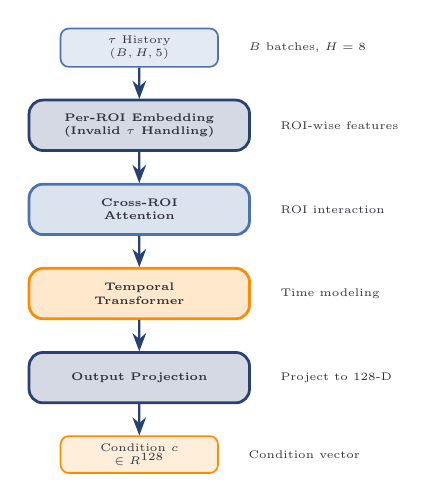
\begin{tikzpicture}[node distance=0.5cm, scale=0.8, transform shape]
    
    % Input
    \node[box=secondary, minimum width=2.5cm] (input) {$\tau$ History\\$(B, H, 5)$};
    
    % Per-ROI embedding
    \node[bigbox=primary, below=of input, minimum width=3.5cm, minimum height=0.8cm] (embed) {Per-ROI Embedding\\(Invalid $\tau$ Handling)};
    
    % Cross-ROI attention
    \node[bigbox=secondary, below=of embed, minimum width=3.5cm, minimum height=0.8cm] (spatial) {Cross-ROI\\Attention};
    
    % Temporal transformer
    \node[bigbox=accent, below=of spatial, minimum width=3.5cm, minimum height=0.8cm] (temporal) {Temporal\\Transformer};
    
    % Output projection
    \node[bigbox=primary, below=of temporal, minimum width=3.5cm, minimum height=0.8cm] (proj) {Output Projection};
    
    % Output
    \node[box=accent, below=of proj, minimum width=2.5cm] (out) {Condition $c$\\$\in \mathbb{R}^{128}$};

    % Short block explanations
    \node[anno, anchor=west] at ($(input.east)+(0.35,0)$) {$B$ batches, $H=8$};
    \node[anno, anchor=west] at ($(embed.east)+(0.35,0)$) {ROI-wise features};
    \node[anno, anchor=west] at ($(spatial.east)+(0.35,0)$) {ROI interaction};
    \node[anno, anchor=west] at ($(temporal.east)+(0.35,0)$) {Time modeling};
    \node[anno, anchor=west] at ($(proj.east)+(0.35,0)$) {Project to 128-D};
    \node[anno, anchor=west] at ($(out.east)+(0.35,0)$) {Condition vector};
    
    % Arrows
    \draw[arrow] (input) -- (embed);
    \draw[arrow] (embed) -- (spatial);
    \draw[arrow] (spatial) -- (temporal);
    \draw[arrow] (temporal) -- (proj);
    \draw[arrow] (proj) -- (out);
    
\end{tikzpicture}
\end{center}

\vspace{0.2cm}

\begin{columns}[T]
\begin{column}{0.45\textwidth}
\textbf{\small Key Features}
\begin{itemize}\setlength{\itemsep}{1pt}
    \item[\tiny$\bullet$] \footnotesize Learned embedding for invalid $\tau = -1$
    \item[\tiny$\bullet$] \footnotesize Multi-head attention (4 heads)
    \item[\tiny$\bullet$] \footnotesize 2 transformer layers
\end{itemize}
\end{column}

\begin{column}{0.5\textwidth}
\textbf{\small Dimensions}
\begin{itemize}\setlength{\itemsep}{1pt}
    \item[\tiny$\bullet$] \footnotesize Embed dim: 32 per ROI
    \item[\tiny$\bullet$] \footnotesize Hidden dim: 128
    \item[\tiny$\bullet$] \footnotesize Output dim: 128
\end{itemize}
\end{column}
\end{columns}
\end{frame}

%===============================================================================
% SLIDE 4: Diffusion Policy - U-Net Denoiser
%===============================================================================
\begin{frame}
\frametitle{\textbf{Diffusion Policy: Conditional 1D U-Net}}
\vspace{-0.3cm}
\begin{center}
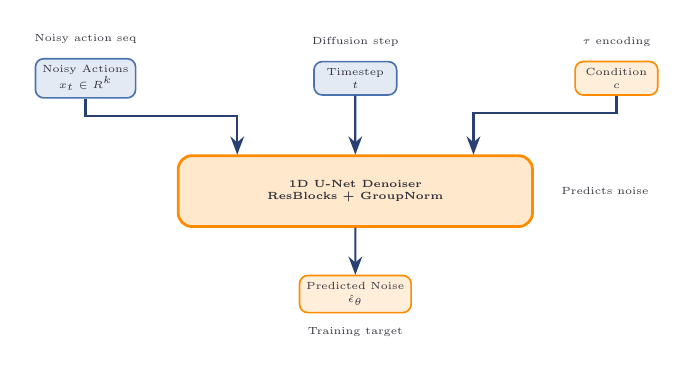
\begin{tikzpicture}[node distance=0.4cm and 1cm, scale=0.75, transform shape]
    
    % Inputs
    \node[box=secondary] (noise) {Noisy Actions\\$x_t \in \mathbb{R}^k$};
    \node[box=secondary, right=3cm of noise] (time) {Timestep\\$t$};
    \node[box=accent, right=3cm of time] (cond) {Condition\\$c$};
    
    % U-Net
    \node[bigbox=accent, below=1cm of time, minimum width=6cm, minimum height=1.2cm] (unet) {
        1D U-Net Denoiser\\
        ResBlocks + GroupNorm
    };
    
    % Output
    \node[box=accent, below=0.8cm of unet] (out) {Predicted Noise\\$\hat{\epsilon}_\theta$};

    % Short block explanations
    \node[anno, above=0.12cm of noise] {Noisy action seq};
    \node[anno, above=0.12cm of time] {Diffusion step};
    \node[anno, above=0.12cm of cond] {$\tau$ encoding};
    \node[anno, anchor=west] at ($(unet.east)+(0.35,0)$) {Predicts noise};
    \node[anno, below=0.12cm of out] {Training target};
    
    % Arrows
    \draw[arrow] (noise.south) -- ++(0,-0.3) -| ($(unet.north)+(-2,0)$);
    \draw[arrow] (time) -- (unet);
    \draw[arrow] (cond.south) -- ++(0,-0.3) -| ($(unet.north)+(2,0)$);
    \draw[arrow] (unet) -- (out);
    
\end{tikzpicture}
\end{center}

\vspace{0.3cm}

\begin{columns}[T]
\begin{column}{0.32\textwidth}
\textbf{\small Training}
\begin{itemize}\setlength{\itemsep}{1pt}
    \item[\tiny$\bullet$] \footnotesize Loss: $\|\epsilon - \hat{\epsilon}_\theta\|^2$
    \item[\tiny$\bullet$] \footnotesize Cosine $\beta$ schedule
    \item[\tiny$\bullet$] \footnotesize $T = 100$ steps
    \item[\tiny$\bullet$] \footnotesize EMA decay: 0.995
\end{itemize}
\end{column}

\begin{column}{0.32\textwidth}
\textbf{\small Inference}
\begin{itemize}\setlength{\itemsep}{1pt}
    \item[\tiny$\bullet$] \footnotesize $T' = 10$ steps (fast)
    \item[\tiny$\bullet$] \footnotesize DDPM sampling
    \item[\tiny$\bullet$] \footnotesize Latency: $<$50ms
\end{itemize}
\end{column}

\begin{column}{0.32\textwidth}
\textbf{\small Action Chunking}
\begin{itemize}\setlength{\itemsep}{1pt}
    \item[\tiny$\bullet$] \footnotesize Predict $k=8$ actions
    \item[\tiny$\bullet$] \footnotesize Execute 4, replan
    \item[\tiny$\bullet$] \footnotesize Smoother control
\end{itemize}
\end{column}
\end{columns}

\vspace{0.2cm}
\centering
\textbf{\small Total Parameters:} $\sim$500K
\end{frame}

%===============================================================================
% SLIDE 5: Ablation Study Design
%===============================================================================
\begin{frame}
\frametitle{\textbf{Experimental Design: Ablation Study}}
\vspace{-0.2cm}

\begin{center}
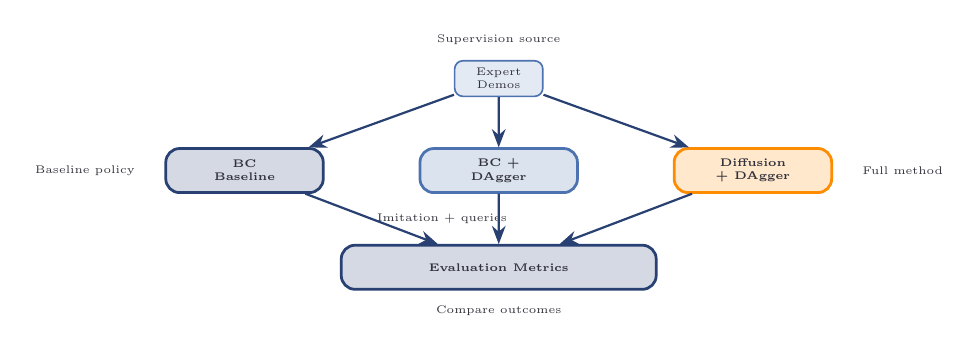
\begin{tikzpicture}[scale=0.8, transform shape]
    
    % Three branches
    \node[bigbox=primary, minimum width=2.5cm] (bc) {BC\\Baseline};
    \node[bigbox=secondary, right=1.5cm of bc, minimum width=2.5cm] (bcd) {BC +\\DAgger};
    \node[bigbox=accent, right=1.5cm of bcd, minimum width=2.5cm] (diff) {Diffusion\\+ DAgger};
    
    % Arrows from common source
    \node[box=secondary, above=0.8cm of bcd] (data) {Expert\\Demos};
    
    \draw[arrow] (data) -- (bc);
    \draw[arrow] (data) -- (bcd);
    \draw[arrow] (data) -- (diff);
    
    % Evaluation
    \node[bigbox=primary, below=0.8cm of bcd, minimum width=5cm] (eval) {Evaluation Metrics};

    % Short block explanations
    \node[anno, anchor=east] at ($(bc.west)+(-0.35,0)$) {Baseline policy};
    \node[anno, anchor=north] at ($(bcd.south)+(-0.9,-0.2)$) {Imitation + queries};
    \node[anno, anchor=west] at ($(diff.east)+(0.35,0)$) {Full method};
    \node[anno, above=0.12cm of data] {Supervision source};
    \node[anno, below=0.12cm of eval] {Compare outcomes};
    
    \draw[arrow] (bc) -- (eval);
    \draw[arrow] (bcd) -- (eval);
    \draw[arrow] (diff) -- (eval);
    
\end{tikzpicture}
\end{center}

\vspace{0.3cm}

\begin{columns}[T]
\begin{column}{0.45\textwidth}
\textbf{\small Methods Compared}
\begin{enumerate}\setlength{\itemsep}{2pt}
    \item \footnotesize BC: Simple MLP baseline
    \item \footnotesize BC + DAgger: With expert queries
    \item \footnotesize \textbf{Diffusion + DAgger}: Full method
\end{enumerate}
\end{column}

\begin{column}{0.5\textwidth}
\textbf{\small Evaluation Metrics}
\begin{itemize}\setlength{\itemsep}{1pt}
    \item[\tiny$\bullet$] \footnotesize Success rate (\%)
    \item[\tiny$\bullet$] \footnotesize Collision count
    \item[\tiny$\bullet$] \footnotesize Path length ratio
    \item[\tiny$\bullet$] \footnotesize Trajectory smoothness
\end{itemize}
\end{column}
\end{columns}
\end{frame}

\end{document}
